\chapter{Deep Learning}

\section{Neural Networks}

\hspace{0.5cm}A neural network is a set of algorithm that attempt to expose the underlying relationships in data set through a process that inspired by the way human brain operates. A neural network is a combination of a set highly interconnected computational unit called \textit{neurons}. The diagram below shows a comparison of structure between a biological neural (left) and a neurons in neural network.
\begin{figure}[h!]
    \centering
    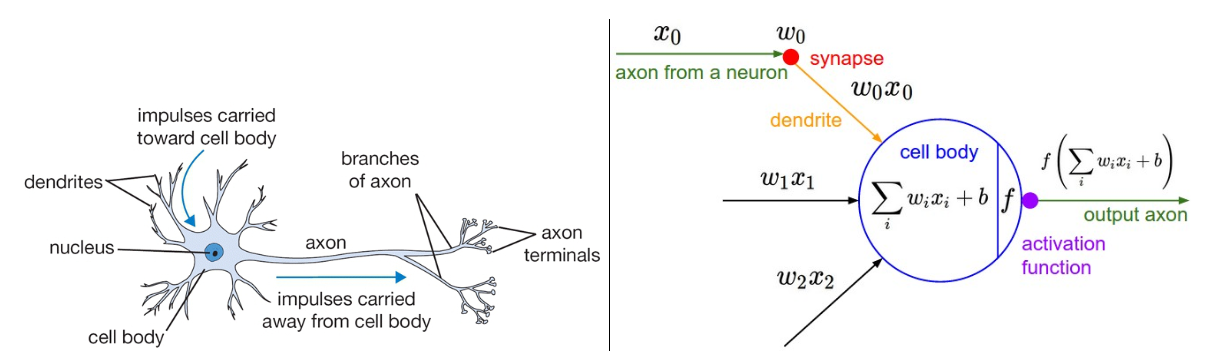
\includegraphics[width=0.9\textwidth]{Chapters/Fig/neural_arc.PNG}
    \caption{Biological neural (left) and a neurons in Neural Network (right) by CS231n course}
    \label{fig:nn_arc}
\end{figure}
Biological neural receives signal for its denrites and generate the output signals onward its axon. In the mathematical neuron unit, input $x_0$ for other neuron combines multiplicatively (e.g $w_0x_0$ )with the dendrites based on the synaptic strength (e.g $w_0$) corresponding to that synapse.\\
In neural network, synaptic strength $w$ can be updated to control the influence strength of input from another neurons in neural network. The activation function $f$ controls the input by calculated a weighted sum of input, add bias and decides whether is should be fired or not.
\subsection{Activation functions}
\begin{itemize}
    \item \textbf{Sigmoid} a non-linearity function defined as $\sigma(x)=\frac{1}{1 + e^{-x}}$ with diagram in fig.\ref{fig:sigmoid}. This function normalizes the input to range between [0,1]. Sigmoid is used to be frequently used but rarely now because of two major drawbacks: saturating, killing the gradients and not zero-centered outputs.\\
    \begin{figure}[h!]
        \centering
        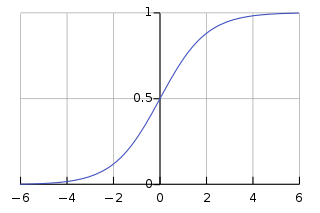
\includegraphics[width=0.4\textwidth]{Chapters/Fig/sigmoid.png}
        \caption{The logistic curve by Wikipedia}
        \label{fig:sigmoid}
    \end{figure}\\
    The derivative of sigmoid function is calculated as:
    \begin{center}
        \begin{equation}
            \begin{split}
                \frac{d\sigma(x)}{dx} & = (\frac{1}{1+e^{-x}})^2\frac{d}{dx}(1+e^{-x})\\
                                    & = (\frac{1}{1+e^{-x}})(\frac{e^{-x}}{1+e^{-x}})\\
                                    & = [1-\sigma(x)]\sigma(x)
            \end{split}
        \end{equation}
    \end{center}
    \pagebreak
    \item \textbf{Tanh} a non-linearity hyperbolic function that squashes a real number to the range [-1,1]. It zero-centers the output, however,it also saturate the gradients as Sigmoid activation function. The tanh function is defined as:
    \begin{equation}
        \text{tanh}(x) = \frac{e^x - e^{-x}}{e^x + e^{-x}} = 2\sigma(2x) - 1
    \end{equation}
    with the derivative is computed as:
    \begin{equation}
        \frac{d\text{tanh(x)}}{dx} = 1-\text{tanh}^2(x)
    \end{equation}
    The graph of the tanh activation function shown in fig.\ref{fig:tanh}
    \begin{figure}[h!]
        \centering
        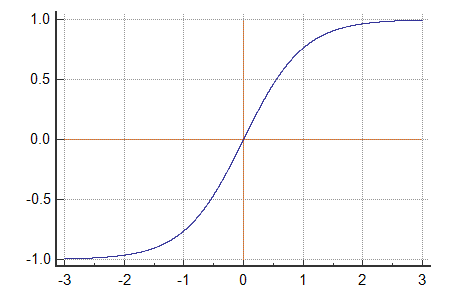
\includegraphics[width=0.4\textwidth]{Chapters/Fig/tanh.png}
        \caption{Tanh activation function}
        \label{fig:tanh}
    \end{figure}

    \item \textbf{ReLU} The Rectified Linear Unit graph of which shown in fig.\ref{fig:relu} computes 
    \begin{equation}
        f(x) = max(0,x)
    \end{equation}
    It has been widely used in the last few years because it more highly accelerates the convergence of stochastic gradient descent than sigmoid/tanh functions due to its linear, non-saturating form. Moreover, implementation of ReLU is easier than sigmoid/tanh functions by simply thresholding a matrix of activations at zero. However, ReLU units can be fragile during training and can die [cs231n]
    \begin{figure}[th!]
        \centering
        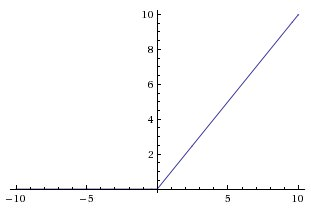
\includegraphics[width=0.4\textwidth]{Chapters/Fig/relu.jpg}
        \caption{The graph of ReLU}
        \label{fig:relu}
    \end{figure}\\
    The derivative of ReLU is:
    \begin{equation}
        \frac{df}{dx} = \begin{cases}
            1 & x < 0\\
            0 & \mbox{otherwise}
        \end{cases}
    \end{equation}
    \item \textbf{Leaky ReLU} is proposed to fix the "dying ReLU" by having a small slope for negative values instead of zero.
        \begin{equation}
        \frac{df}{dx} = \begin{cases}
            1 & x < 0\\
            \alpha x & \mbox{otherwise}
        \end{cases}
    \end{equation}
    where $\alpha$ is a small constant
    \begin{figure}[h!]
        \centering
        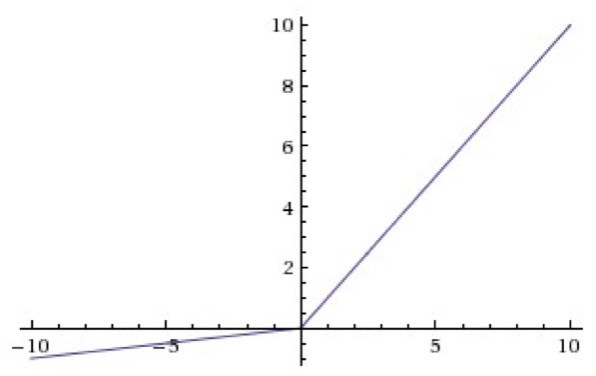
\includegraphics[width=0.4\textwidth]{Chapters/Fig/leaky.jpeg}
        \caption{The graph of Leaky ReLU}
        \label{fig:lrelu}
    \end{figure}
\end{itemize}

\section{Deep Forward Networks}
\hspace{0.5cm} Deep forward networks or feedforward neural networks or multilayer perceptrons are the foundation of most deep learning models. The main goal of feedforward network is to approximate some function $f*$. For example, for a regression, $y = f*(x)$ maps an input x to a value y. A feedforward network defines a mapping $y = f(x;\theta)$ and learns the value of the parameters $\theta$ that result in the best function approximation.\par
These model are called feedforward since the data runs through the mapping from $x \rightarrow y$ to define $f$ without any feedback connections in which outputs of the model are fed back into itself. In a special case, there exists feedback connections in the network, they are called recurrent neural networks which is not presented in this work.
\pagebreak

\subsection{The architecture}
The architecture of the structure of the network refers to the number of hidden layers and the number of hidden units or neurons in each layer. The term network in the name of these models means that they can be represented as a combination of many different functions. For example, suppose we have 3 functions $f^{(1)}$, $f^{(2)}$ and $f^{(3)}$ connected into a chain to form the mapping $f(x) = f^{(3)}(f^{(2)}(f^{(1)}(x))$. In this example, $f^{(1)}$ is called the first layer of the network, $f^{(2)}$ is called the second layer and so on. The final layer is called output layer while the layers between the input and output layers are called hidden layers because the training data does not show the desired output for each of these layers. The length of the chain defines the depth of the network
\begin{figure}[h!]
    \centering
    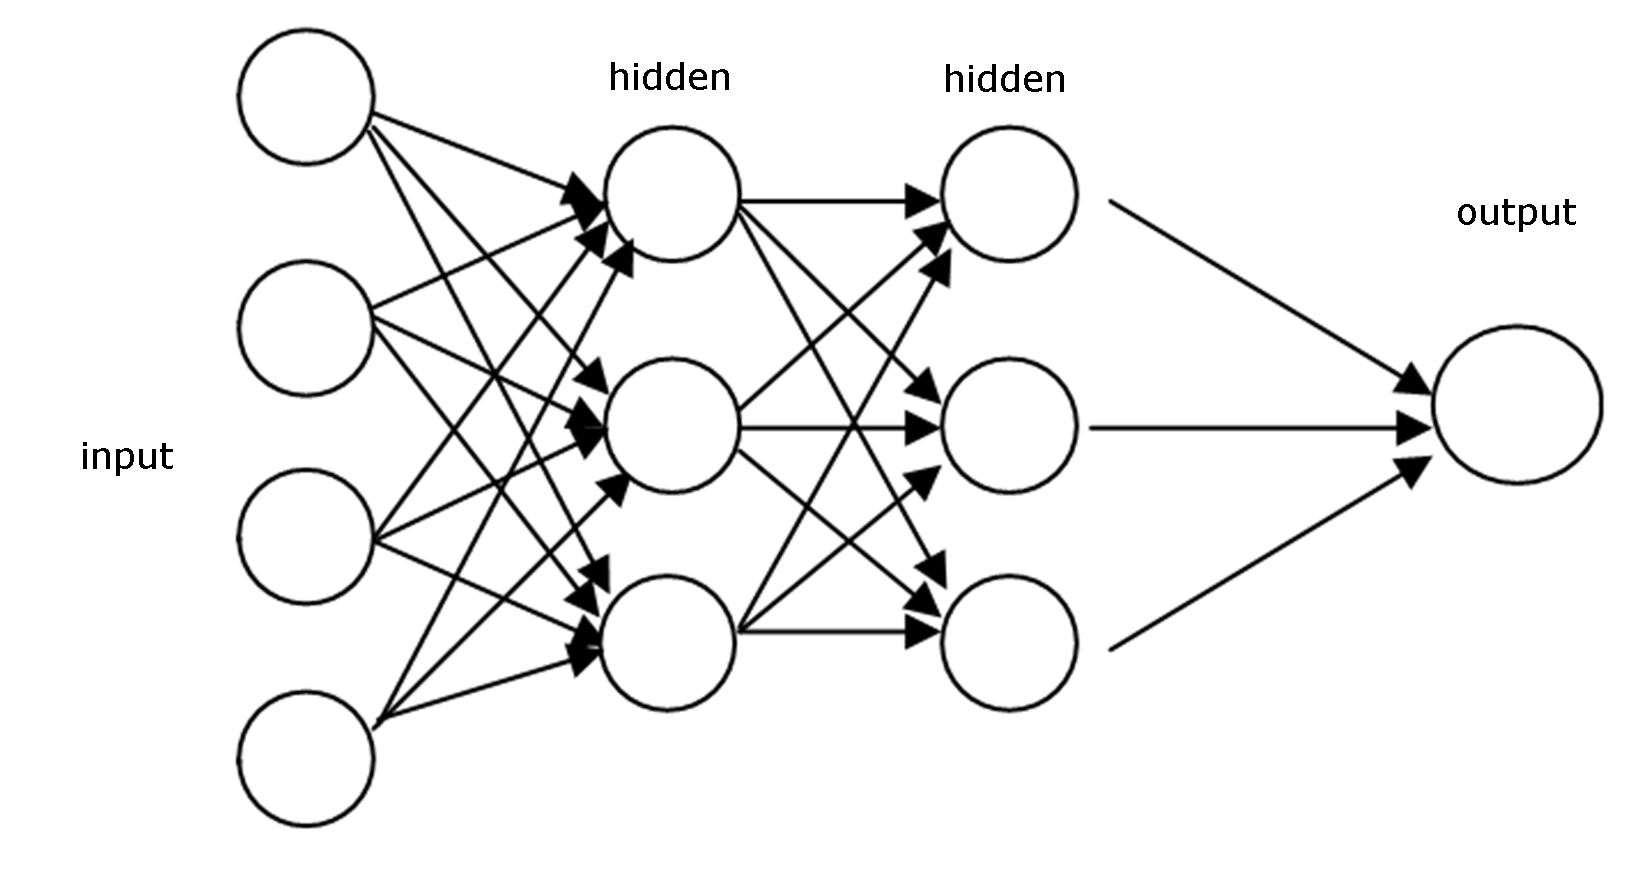
\includegraphics[width=0.6\textwidth]{Chapters/Fig/architecture_mlp.png}
    \caption{Architecture of a simple feedforward neural network}
    \label{fig:arch_mlp}
\end{figure}
\par Fig.\ref{fig:arch_mlp} describes a architecture of a simple feedforward neural network which has two hidden layers which 3 nodes for each hidden layers.
\subsection{Training a Neural Network}
\hspace{0.5cm}Designing and training a neural network are really similar to any other gradient-based learning model. However, the most different property between the linear models and and the neural networks is non-convex loss functions due the the non-linearity of the neural network. Consequently, we have to train the neural network iteratively when the optimizers only decrease the value of the cost function without guarantee of convergence.\par Gradient-based optimizers such as stochastic gradient descent for non-convex loss function are sensitive to the initial value of parameters. For feedforward neural networks. it is important to initialize all weights to small random values while the biases should be zero or small positive values.\par
To apply gradient-based learning in neural network, as same as the other machine learning models, we must choose a cost function for the model, and how the model present its output.
\subsection{Cost functions}
The loss functions $\mathcal{L}$ or the cost function, the objective function or error function used to train a neural network is a measurement of how well the network predicts desired output $\hat{y}$ with given input $x$ compared to the ground truth $y$. Let discuss some of common loss functions:
\begin{itemize}
    \item \textbf{Learning Conditional Distributions with Maximum Likelihood}:
    Most modern network network are trained using maximum likelihood. The cost function in this case is simply negative log-likelihood or the cross-entropy between the training data and model distributions which is defined as:
    \begin{equation}
        J(\theta) = \frac{1}{2}\mathbb{E}_{x,y\sim\hat{p}_{data}}||y-f(x,\theta)||^2 + const
     \end{equation}
     An advantages of this approach is that it avoid the saturate gradient, its gradient is large and predictable to serve as a good guide for the learning algorithm.
     
     \item \textbf{Learning Conditional Statistic}: Learning just one conditional statistic of $y$ given $s$ rather than learning a full probability distribution $p(y|x,\theta )$. Now, the cost function is viewed as a \textit{functional} that is a mapping from functions to real number rather than just a functions. Usually, in most neural network model, the cost function that aims to learn conditional statistic is designed to have its minimum lie on the function that maps $x$ to the expected value of $y$ given x. We use \textit{calculus of variations} to solve the problem of optimization with respect to a function. These two results obtained from the mentioned above technique for optimization problems:
     \begin{itemize}
         \item Mean-squared error function:
         \begin{equation}
             f^* = \underset{f}{\mathrm{argmin}}\mathbb{E}_{x,y\sim p_{data}}||y-f(x)||^2
         \end{equation}
         \item Mean-absolute error function:
         \begin{equation}
             f^* = \underset{f}{\mathrm{argmin}}\mathbb{E}_{x,y\sim p_{data}}||y-f(x)||_1
         \end{equation}
     \end{itemize}
     Unfortunately, some output units when combine with mean-squared error and mean-absolute functions lead to very small gradients which cause poor result when used these two cost functions with gradient-based optimizations. This is one of the reasons that cross-entropy loss is more frequently used that these two mentioned cost functions, even in case of estimating conditional statistic. 
\end{itemize}
\subsection{Output units}
Choosing a cost function for the models is closely tied together with choosing a output unit. Assume that we choose the cross-entropy cost functions then the choice of output unit is the way the model represent the output then form the cross- entropy function.\par
\begin{itemize}
    \item \textbf{Linear units for Gaussian output distributions}: Linear output layers are often used to produce the mean of a conditional Gaussian distribution:
    \begin{equation}
        p(y|x;\theta) = \mathcal{N}(y|f(x;\theta, \mathbf{I}))
    \end{equation}
    where $\mathbf{I}$ is the co variance matrix which is independent of $\theta$\\
    Maximizing the log-likelihood is equivalent to minimizing the mean-squared error, then, the loss function is formed as:
    \begin{equation}
        \mathcal{L}(\theta) = \frac{1}{2}\underset{i=1}{\overset{N}{\Sigma}}||f(x^{(i)};\theta) - y^{(i)}||^2
    \end{equation}
    \item \textbf{Sigmoid units for Bernoulli output distribution}: Consider the binary classification in which outputs are $\mathcal{C}_1$ or $\mathcal{C}_2$.
    This maximum-likelihood method is to define Bernoulli distribution which is defined by just a single number over $y$ conditioned by $x$. The model tries to predict $P(y=1|x)$ defined as:
    \begin{equation}
        P(y=1|x) = max\{0, min\{1, w^Th+b\}\}
    \end{equation}
    However, it is unable to train it effectively with gradient descent, hence, we define sigmoid output unit which ensures there is always a strong gradient. Sigmoid output unit is defined by:
    \begin{equation}
        \hat{y} = \sigma(w^Th + b)
    \end{equation}
    then when we have a binary cross-entropy error function is formed as:
    \begin{equation}
        \mathcal{L}(\theta) = -\frac{1}{N}\underset{i=1}{\overset{N}{\Sigma}}y_i*log(\hat{y}_i) + (1-y_i)*log(1-\hat{y}_i)
    \end{equation}
    \item \textbf{Softmax output units for Multinoulli output distribution}:When we want output of the model to present a probability distribution over a discrete variable of $n$ possible values, softmax output unit is considerable choice. The output $y$ is written under 1-of-\textbf{C} codeing scheme such that $c = 1,...,C$ are the class labels, the outputs of the networks now are viewed as $f^{k}(x,\theta) = p(y^{k}=1|x)$, leading to the \textit{categorical cross-entropy} loss function:
    \begin{equation}
        \mathcal{L}(\theta) = - \underset{i=1}{\overset{N}{\sum}}\underset{c=1}{\overset{C}{\sum}}y^{(c)(i)}\text{log}f^{(k)}(x^{(i)};\theta)
    \end{equation}
\end{itemize}
\subsection{Parameters optimization}
\hspace{0.5cm}The purpose of a neural network is to learn to recognize patterns of the data.Once a neural network has been trained well, it is able to predict an output $\hat{y}$ given input $x$ that is close to the ground truth $y$. We can say, training a neural network is a process of optimizing the parameters $\theta$ for the mapping $\hat{y} : f(x;\theta)$ with the minimal difference between $\hat{y}$ and $y$.\par
Before discuss more about the optimization problem, let's clarify terminologies and notations:\par
Assume $f(x)$ is the function that is going to be minimized
\begin{itemize}
    \item The \textit{derivative} of $f(x)$, denoted as $f'(x)$ or $\frac{\text{d}f}{\text{d}x}$, is the slope of $f(x)$ at point $x$. The \textit{derivative} of $f(x)$ measures how sensitive of change in $x$ to the change in $f(x)$
    \item If the input $\pmb{x}$ is multi dimensional, the \textit{partial derivative} of $f(x)$, denoted as $\frac{\partial f}{\partial x_i}$, measures how $f$ changes if $x_i$ in $x$ changes.
    \item The set of all \textit{partial derivative} of $f(\pmb{x})$ called gradient of $f$ denoted by $\nabla_{\pmb{x}} f(\pmb{x})$
\end{itemize}
\par We mentioned the term \textit{gradient-based learning} or \textit{gradient descent} in about sections, then, we discuss more detail about this optimization technique. Gradient descent (GD) is used for minimizing the loss function $\mathcal{L}(\theta)$ by continuously subtracting value of the gradient $\mathcal{L}(\theta)$ from $\theta$ with respect to $\theta$. In each iteration $t$ of training process, the update rule of GD is:
\begin{equation}
    \theta_t = \theta_{t-1} - \eta . \frac{1}{N}\nabla_{\theta}\mathcal{L}\theta
\end{equation}
where $N$ is the number of examples in training set, $\eta$
\par By iteratively moving in the direction of steepest descent or the gradient which tell us the direction of the slope of the loss function  $\mathcal{L}$, we can find an optimization $\theta$ which enable the network can predict more accurately.\par
Computing the gradient descents by going through all samples in the training set iteratively causes a very expensive computational cost for large scale datasets. To tackle this problem, there are several improvements of vanilla GD:
\begin{itemize}
    \item \textbf{Mini-batch gradient descent} (MGD): Instead of computing the full loss function over the entire training set in order to perform only a single parameter update, this technique computes the gradient over batches of the training data.
    \item \textbf{Stochastic gradient descent} (SGD): The extreme case of mini-batch gradient descent where the mini-batch size is one. In practical, vectorized code optimizations can be computationally much more efficient to evaluate the gradient for 100 examples rather than the gradient for one example 100 times. However, people use the term \textit{SGD} when referring to mini-batch gradient descend, where it is usually assumed that mini-batches are used.
\end{itemize}
\subsection{Back-propagation algorithm}
\hspace{0.5cm}The input $\pmb{x}$ provide the initial information that then flow forward up the hidden unit in each layer and finally output $\hat{\pmb{y}}$, the process called \textit{forward propagation}. The \textit{back-propagation} algorithm, or simply called backprop, allows the information from the cost function to propagate backwards throught in order to compute the gradient.\par
The term back-propagation is often misunderstood as the learning technique for multi-layer neural network while back-propagation is only a method for computing the gradient, and techniques like SGD is used to perform learning using the gradient.\par
Backprop algorithm computes gradient using the chain rule of calculus which is defined as a technique to compute the the derivatives of functions formed by composing other functions whose derivatives are known. Suppose that $y=g(x)$ and $z = f(g(x)) = f(y)$ the the chain rule states that:
\begin{equation}
    \frac{\text{d}z}{\text{d}x}  = \frac{\text{d}z}{\text{d}y}\frac{\text{d}y}{\text{d}x}
\end{equation}\par
In a multilayer neural network, each neural computes a weighted sum of its input formed as
\begin{equation}
    a_j = \underset{i}{\sum}w_{ji}z_i
\end{equation}
where $z_i$ output of node $i^{th}$ that is the input of the node $j^{th}$; $w_{ij}$ is the weight associated with the connection. The $a_j$ is going through the activation function $f$ to produce output of the $j^{th}$
node described as:
\begin{equation}
    z_j = f(a_j)
\end{equation}
Then, the derivative of $\mathcal{L}_n$ corresponding to the a weight $w_{ij}$ is calculated by applying chain rule is described as follow:
\begin{equation}
    \frac{\partial \mathcal{L}_n}{ \partial w_{ij}} = \frac{\partial \mathcal{L}_n}{ \partial a_{j}}\frac{\partial a_{j}}{ \partial w_{ij}}
\end{equation}
Denote $\delta_j$ $\equiv$ $\frac{\partial \mathcal{L}_n}{ \partial a_{j}}$
\par
Derive from (2.24) we have:
\begin{equation}
    \frac{\partial a_j}{ \partial w_{ij}} = z_i
\end{equation}
then, the partial derivative of $\mathcal{L}_n$ corresponding to weight $w_{ij}$ in (2.26) can be obtained as:
\begin{equation}
    \frac{\partial \mathcal{L}_n}{ \partial w_{ij}} = \delta_j z_i
\end{equation}
\par For output neuron, $\delta_{out}$ is computed as:
\begin{equation}
    \delta_{out} = y^{(k)} - \hat{y}^{(k)}
\end{equation}
For each hidden neuron $j$, the value of $\delta_j$ is evaluated follow:
\begin{equation}
    \begin{split}
        \delta_j & \equiv \frac{\partial \mathcal{L}_n}{ \partial a_{j}} = \underset{k}{\sum}\frac{\partial \mathcal{L}_n}{ \partial a_{k}}\frac{\partial a_k}{ \partial a_{j}}\\
                        &\hspace{1.4cm} = f'(a_j)\underset{k}{\sum}w_{kj}\delta_k
    \end{split}
\end{equation}
where the sum is calculated over all neurons $k$ that are connected from neuron $j$\par
The equation (2.30) indicates the value of $\delta$ for a particular hidden neural by propagating the $\delta$'s backwards from neurons in the previous layer of the network. Because the value of $\delta$ for output layer is straight forward, the $\delta$'s can be computed by recursively applying equation (2.30) for all neurons in hidden layers of a feedforward neural network. Therefore, the partial derivatives of the loss function $\mathcal{L}$ to every weight in the network can be obtained by using backprop.
\subsection{Summary}
\hspace{0.5cm} By defining the conceptions and algorithms in above sections, we can briefly describe the process of training a neural network with mini-batch gradient descend technique applied back-propagation algorithm. There are two main phases of training process:
\begin{itemize}
    \item \textbf{Forward pass}
    \begin{itemize}
        \item Forward the input $\pmb{x}$ sample to obtain the activation for hidden layers and output layer
        \item Calculate the loss between the predicted output $\hat{y}$ and the ground truth $y$
    \end{itemize}
    \item \textbf{Backward pass}
    \begin{itemize}
        \item Back propagate the loss from the output layer, through out all the hidden layers to the input layers to acquire the partial derivatives of the loss function corresponding to all the weight of the network
        \item Then, update each weight using MGD update rules.
    \end{itemize}
\end{itemize}\par
The stopping criteria of the training process is based on the convergence of the loss function or the number of training iteration exceeds a predefined threshold.

\section{Convolutional Neural Network}
\hspace{0.5cm}
Convolutional neural network or CNN which is firstly introduced in \cite{cnn} is a variant of FNN specialized 
for processing data which is grid-like topology. For example, time-series data which can be presented as 1D grid 
taking samples at regular time intervals, or image data which can be thought as a 2D of pixels values. Convolutional neural networks have proved how effective they are in practicals problems. 
The name \textit{Convolutional neural network} demonstrates that a neural network employs a mathematical operation called \textit{convolution}.\par
With high-dimensional data, ordinary neural network shows up the disadvantage that all the number of parameters add up quickly and simultaneously with the number of dimensional of the data. For example, with a image size 200x200x3, we expect a neuron should have 200*200*3 = 120,000 weights. Obviously, full connectivity is wasteful and the huge number of parameters would rapidly lead to over-fitting.\par
CNN was proposed to overcome this problem by combining three architectural ideas: \textit{local receptive field},\textit{parameter sharing} and spatial or temporal \textit{sub-sampling}. The general architecture of a CNN is a combination of convolutional layers stacked together with non-linear layers and pooling layers between.
\subsection{The convolution operation}
\hspace{0.5cm} Convolution is an operation of two functions of a real valued argument. In machine learning applications, the input is usually as multi-dimensional array of data and the kernel is the usually a multi-dimensional array of parameters that are adapted by the learning algorithm. Convolution operation is often used over more than one axis at a time. Suppose there is a two-dimensional image \textit{I} as input and a two-dimensional kernel \textit{K}:
\begin{equation}
    S(i,j) = (I*K)(i,j) = \underset{m}{\sum}\underset{n}{\sum}I(i-m,j-nn)K(m,n)
\end{equation}
\par
Intuitively, the kernel slides to every position of the image and computes a new pixel as a weighted sum of the pixels it floats over. The visualization for the convolution operation in fig.\ref{fig:conv}\footnote{https://colah.github.io}:\par
\begin{figure}[h!]
    \centering
    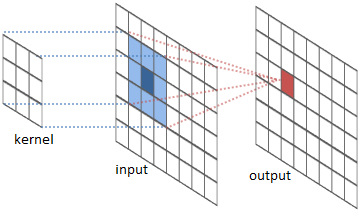
\includegraphics[width=0.5\textwidth]{Chapters/Fig/conv.png}
    \caption{Convolution operation of an image and a kernel}
    \label{fig:conv}
\end{figure}\par
\subsection{Convolutional layer}
\begin{itemize}
    \item \textbf{Local Connectivity} Instead of connect neurons to all neurons in the previous volume. in CNN, we will connect each neuron to only a local region of the input volume. The spatial extent of this connectivity is a hyper parameter called the \textit{receptive field} of the neuron. The connections are local in space (along width and height), but always full along the entire depth of the input volume.
    \begin{figure}[h!]
        \centering
        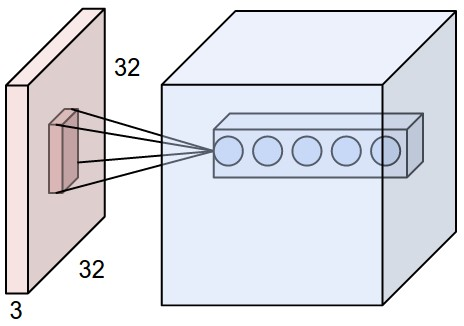
\includegraphics[width=0.3\textwidth]{Chapters/Fig/local_connectivity.jpeg}
        \caption{Local connectivity in CNN. The connection if local in spatial dimension but extends full depth of the input volume}
        \label{fig:local_connect}
    \end{figure}
    \pagebreak
    \item \textbf{Parameter-sharing scheme} Parameter sharing is used in Convolutional layers to control the number of parameters. This technique assumes that if one feature is useful to compute at some spatial position $(x,y)^i$, then is should also be useful to compute at a different position $(x,y)^j$. Denote a single 2-dimensional slice of depth as depth size e.g. for a image with size 200x200x3 has 3 depth slices, each of size [200x200], we are going to constrain the neurons in each depth slide to use the same weights and bias. However, during back-propagation, every neuron in the volume will compute the gradient for its weights, the these gradients will be added up across each depth slice and only update a single set of weight per slice.
    \begin{figure}[h!]
        \centering
        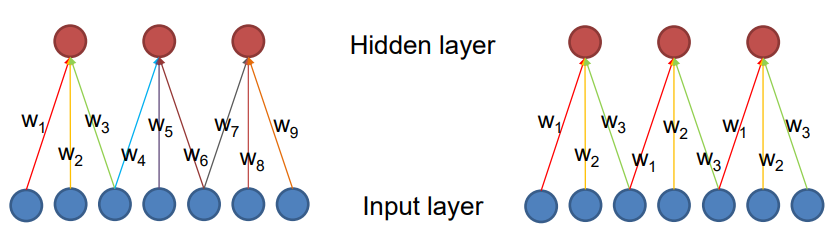
\includegraphics[width=0.8\textwidth]{Chapters/Fig/parameter-sharing.png}
        \caption{Left: without weight sharing, right: with weight sharing}
        \label{fig:param_share}
    \end{figure}
    \item \textbf{Spatial Arrangement} There are three hyperparameters which defines the size of the output volume: the \textit{depth}, the \textit{stride} and the \textit{zero-padding}.
    \begin{itemize}
        \item The depth: the number of the kernels in convolutional layer
        \item The stride: indicate how many pixels the filter is shifted at each step
        \item The zero-padding is a hyperparameter that defines the how many pixels of zero are added around the border of input volumes.
    \end{itemize}
\end{itemize}
In conclusion, a convolutional layer:
\begin{itemize}
    \item accepts an input volume of size $W_1$x$H_1$x$D_1$
    \item Requires four hyperparameters:
    \begin{itemize}
        \item Number of filters $K$
        \item Spatial extend or size of receptive field $F$
        \item The stride $S$
    \end{itemize}
    \item Produces a volume of size $W_2$x$H_2$x$D_2$ where:
    \begin{itemize}
        \item $W_2 = \frac{W1-F + 2P}{S} + 1$
        \item $H_2 = \frac{W2-F + 2P}{S} + 1$
        \item $D_2=K$
    \end{itemize}
    \item With parameter sharing, it introduces $F.F.D2$ weight per filter, for a total of $(F.F.D_1).K$ weights and $K$ bias.
    \item In the output volume, the $d$-th depth slice (of size $W_x$x$H_2$) is the result of performing a valid convolution of the $d$-th filter over the input volume with a stride $S$, and then offset by $d$-th bias.
\end{itemize}
\subsection{Pooling layer}
The pooling layer which usually follows convolutional layers is function to progressively reduce the spatial resolution of the feature map. Moreover, it also reduces the parameters and computation in the network, hence, it can control overfitting. The pooling layer executes independently on every channel of the input volume and resizes it spatially, using \textit{max} or \textit{average} operations. Generally, the pooling layer:
\begin{itemize}
    \item Accepts the volume of size $W_1$x$H_1$x$D_1$
    \item Requires two hyperparameters:
    \begin{itemize}
        \item Spatial extend or size of receptive filed $F$
        \item the stride $S$
    \end{itemize}
    \item Produces a volume of size $W_2$x$H_2$x$D_2$ where:
    \begin{itemize}
        \item $W_2 = \frac{W1-F}{S} + 1$
        \item $H_2 = \frac{W2-F}{S} + 1$
        \item $D_2=K$
    \end{itemize}
    \item Introduces zero parameters because it computes a fixed function of the input
    \item For Pooling layers, it is not common to use the zero padding for the input
\end{itemize}
\subsection{Global Average Pooling}
\hspace{0.5cm}Global Average Pooling (GAP) first proposed in \cite{netinnet} is used to minimize overfitting by reducing the total number of parameters in the model. Similar to ordinary pooling layer, GAP layers are used to reduce the spatial dimensions of multi-dimensional volume. However, GAP layers perform a more extreme type of dimensional reduction. Concretely, suppose there is a input volume with dimensions $h$x$w$x$d$, after forwarding through GAP layer, the output volume would have the dimensions of $1$x$1$x$d$. GAP layers reduce each $h$x$w$ feature map to a single number by simply taking the average of all $h$x$w$ values. The visualization of GAP is shown in fig.\ref{fig:gap}\footnote{https://alexisbcook.github.io}
\begin{figure}[h!]
    \centering
    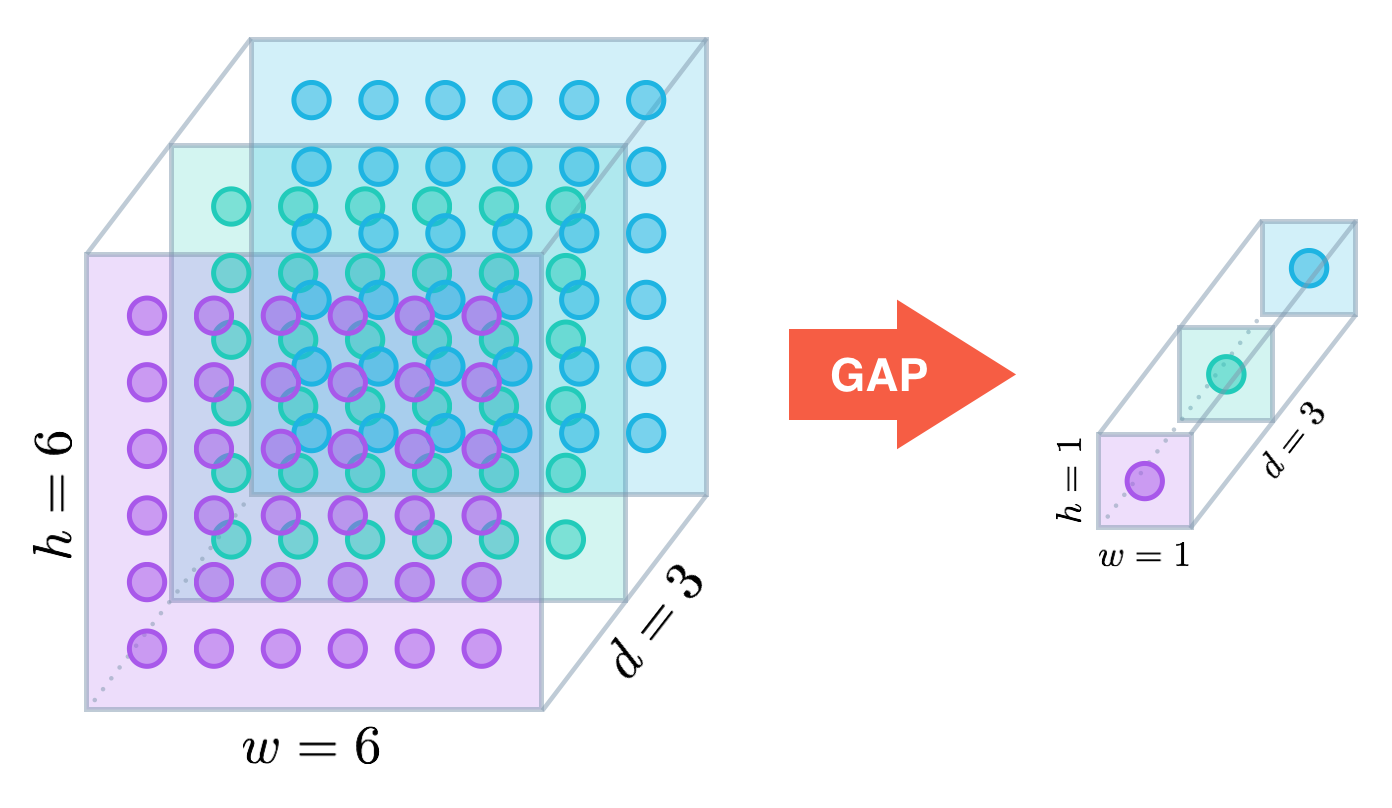
\includegraphics[width=0.5\textwidth]{Chapters/Fig/gap.png}
    \caption{Global Pooling Layer}
    \label{fig:gap}
\end{figure}
\subsection{Fully-connected layer}
\hspace{0.5cm} In fully-connected layer, the neurons have full connections to all activations in the previous layer as same as in ordinary neural network. Therefor, their activations can be computed with a matrix multiplication adding with a bias offset.\par
The output of the last fully-connected layer is often fed into a transformation function mentions in section \textbf{OUTPUT UNITS} which depends on what problems we are solving.
\subsection{Residual block}
\hspace{0.5cm} Network architecture with residual block (ResNet) which is firstly proposed by \cite{He_2016_CVPR} won the ImageNet Visual Recognition Challenge in 2015 and now it becomes as a common approaches to solve several types of problems in Computer Vision. The core idea of ResNet is introducing an \textit{identity shortcut connection} that skips one or more layer shown in fig.\ref{fig:res_block}
\begin{figure}[h!]
    \centering
    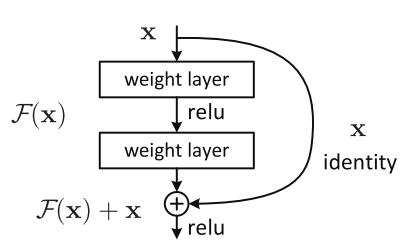
\includegraphics[width=0.6\textwidth]{Chapters/Fig/res_block.png}
    \caption{A residual block}
    \label{fig:res_block}
\end{figure}\par
 The performance of the network is closely related to its depth. Suppose we superimposed several layers on a shallow network A to form a network B, if these newly added layers are \textit{Identity} mapping, the performance of the network B is at least not worse than A. However, the actual experimental results show that the deeper the network, the worse the performance\cite{He_2016_CVPR}, so the author in \cite{He_2016_CVPR} guesses that solver is difficult to learn unit mapping. Since the learning unit mapping is cumbersome, simply add a shortcut to it and directly add the input to the module. In the actual case, the unit map $\pmb{x}$ is not the optimal solution $H(\pmb{x})$, and the optimal solution is near the unit map. The difference between this optimal solution and the unit map is called residual $F(\pmb{x}) = H(\pmb{x}) - \pmb{x}$.\par
 For a very depth network, which has 52 or even hundreds of layers, \cite{He_2016_CVPR} proposed a bottleneck structure for residual block which employs two $1$x$1$ convolution with a $3$x$3$ in the middle shown in fig.\ref{fig:b_res}
 \begin{figure}
     \centering
     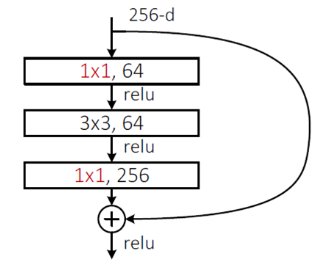
\includegraphics[width=0.5\textwidth]{Chapters/Fig/bottle_neck_residual.PNG}
     \caption{Bottleneck Structure for Residual block}
     \label{fig:b_res}
 \end{figure}
 \par It is effective in reducing number of parameters for very deep neural networks such as ResNet50/101/152.

\pagebreak